\section{Análise preliminar}

Na análise teórica, o comportamento do circuito é considerado tanto para os grandes sinais quanto para os pequenos sinais. São utilizados modelos diferentes para cada um desses casos, conforme detalhado a seguir.

\begin{figure}[H]
    \centering
    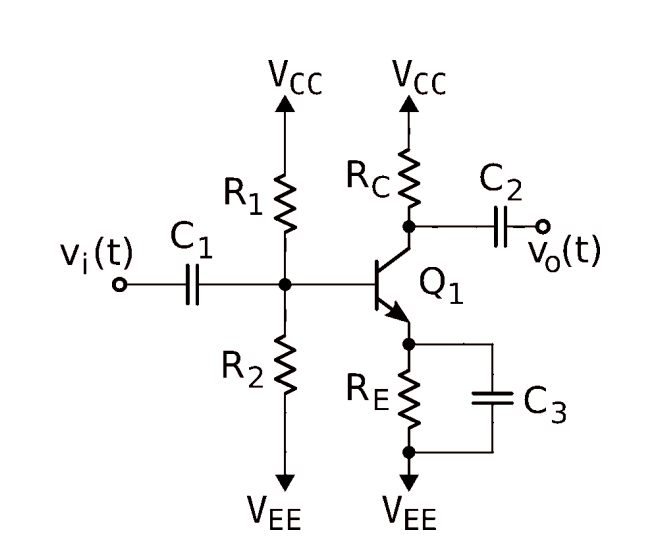
\includegraphics[width=0.5\columnwidth]{images/o_circuito.png}
    \caption{Circuito amplificador emissor de base comum.}
\end{figure}

\subsection{Análise simbólica grandes sinais}

A análise é conduzida, examinando-se as restricoes de polarizacao do transistor e as equacoes de nos do circuito.

Utiliza-se o modelo \ref{fig:modelo_grandes_sinais} para analisar o TBJ quando submetido para grandes sinais.

\begin{figure}[H]
    \centering
    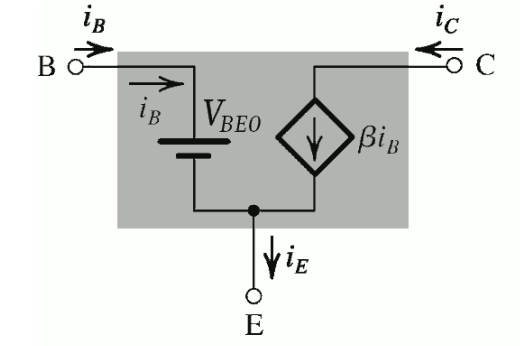
\includegraphics[width=0.5\columnwidth]{images/modelo_grandes_sinais.png}
    \caption{Modelo TBJ para grandes sinais.}
    \label{fig:modelo_grandes_sinais}
\end{figure}

Com este modelo, é possível fazer a substituição no circuito. Para grandes sinais, os capacitores do circuito se comportarão como circuito em aberto, o que permite removê-los na análise, resultando no circuito mostrado na figura \ref*{fig:circuito_grandes_sinais}.

\begin{figure}[H]
    \centering
    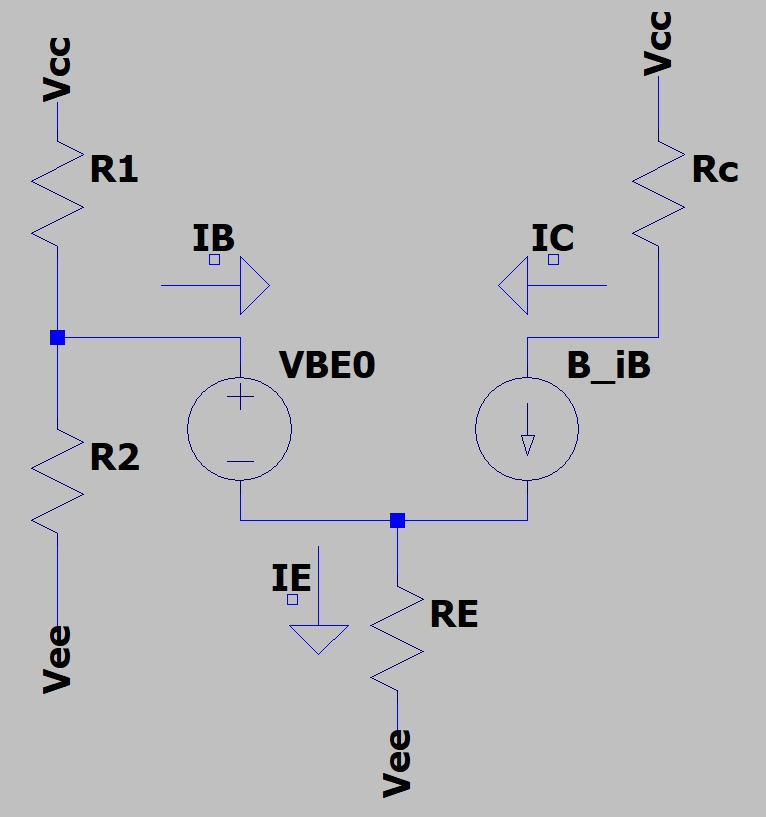
\includegraphics[width=0.3\columnwidth]{images/circuitos_grandes_sinais.png}
    \caption{Circuito com substituições para grandes sinais.}
    \label{fig:circuito_grandes_sinais}
\end{figure}

\subsubsection{Restricões}

Para que o transistor esteja na região ativa, é necessário que sejam satisfeitas as seguintes condições.

\begin{equation}
    \begin{cases}
        V_{BE} = 0.7 V  \\
        V_{CE} > 0.2 V  \\
        I_C = \beta I_B \\
        I_E = I_C + I_B
    \end{cases}
    \label{eq:restricoes_grandes_sinais}
\end{equation}

\subsubsection{Análise nodal do circuito}

Utiliza-se a lei de Kirchhoff das correntes para derivar as equações nodais seguintes.

\begin{equation}
    \begin{aligned}
         & I_{b} + \frac{V_{b} - Vee}{R_{2}} + \frac{V_{b} - Vcc}{R_{1}} = 0 \\
         & \frac{- V_{e} + Vee}{R_{e}} = I_{e}                               \\
         & \frac{- V_{c} + Vcc}{R_{c}} = I_{c}                               \\
    \end{aligned}
    \label{eq:analise_nodal_grandes_sinais}
\end{equation}

\subsubsection{Solução das tensões e correntes}

Utiliza-se as restricoes \ref*{eq:restricoes_grandes_sinais} e as equacoes do circuito \ref*{eq:analise_nodal_grandes_sinais} e resolvemos simbolicamente para $V_b$, $V_c$, $V_e$, $I_b$, $I_c$ e $I_e$.

As equações foram resolvidas utilizando a biblioteca Sympy, e o código correspondente está no apêndice. As soluções das variáveis tornaram-se muito extensas para serem representadas no formato de equações. Portanto, estamos apresentando somente as figuras que ilustram os resultados de cada variável.

\begin{figure}[H]
    \centering
    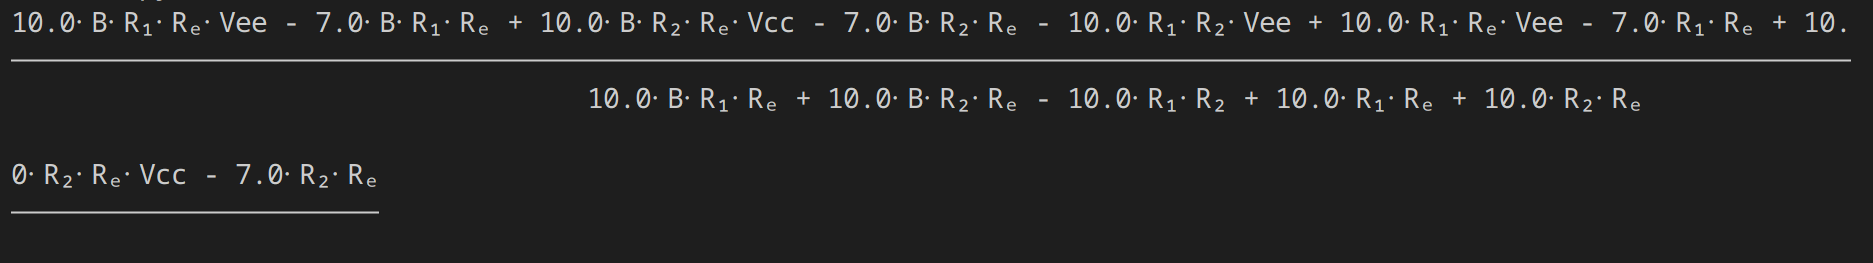
\includegraphics[width=0.7\columnwidth]{images/Ve}
    \caption{Tensão no nó $V_e$.}
\end{figure}

\begin{figure}[H]
    \centering
    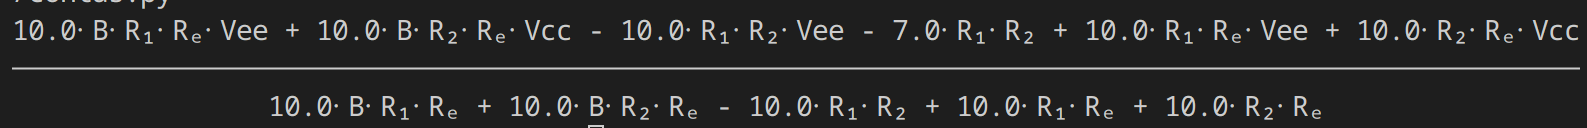
\includegraphics[width=0.7\columnwidth]{images/Vb}
    \caption{Tensão no nó $V_b$.}
\end{figure}

\begin{figure}[H]
    \centering
    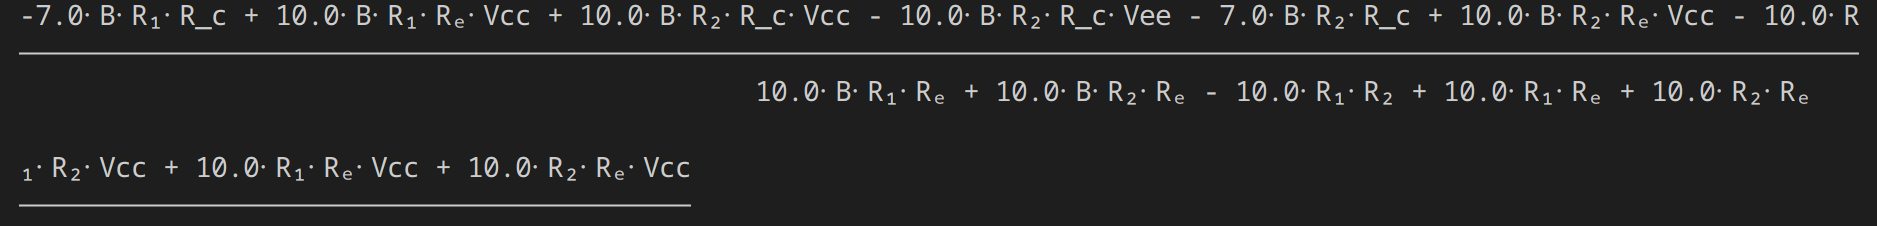
\includegraphics[width=0.7\columnwidth]{images/Vc}
    \caption{Tensão no nó $V_c$.}
\end{figure}

\begin{figure}[H]
    \centering
    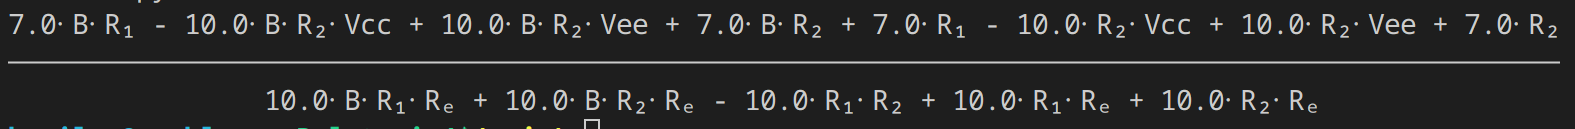
\includegraphics[width=0.7\columnwidth]{images/Ie}
    \caption{Corrente $I_e$.}
\end{figure}

\begin{figure}[H]
    \centering
    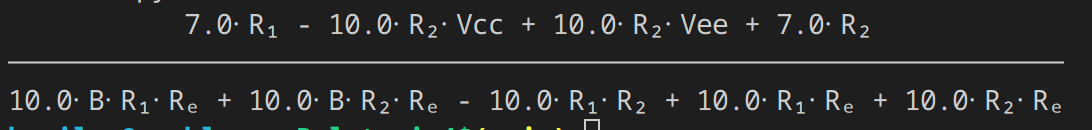
\includegraphics[width=0.7\columnwidth]{images/Ib}
    \caption{Corrente $I_b$.}
\end{figure}

\begin{figure}[H]
    \centering
    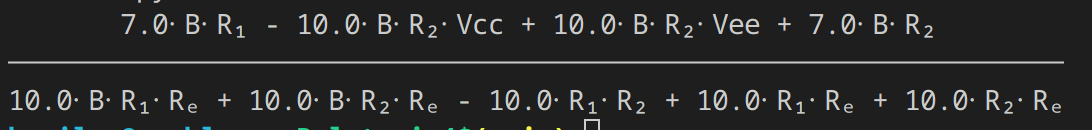
\includegraphics[width=0.7\columnwidth]{images/Ic}
    \caption{Corrente $I_c$.}
\end{figure}

\subsection{Análise simbólica pequenos sinais}

Na análise de pequenos sinais, adotamos a simplificação de considerar que os capacitores se comportam como curtos-circuitos. Além disso, assumimos que todas as fontes de tensão contínua (\emph{DC}) estão devidamente aterradas.

\begin{figure}[H]
    \centering
    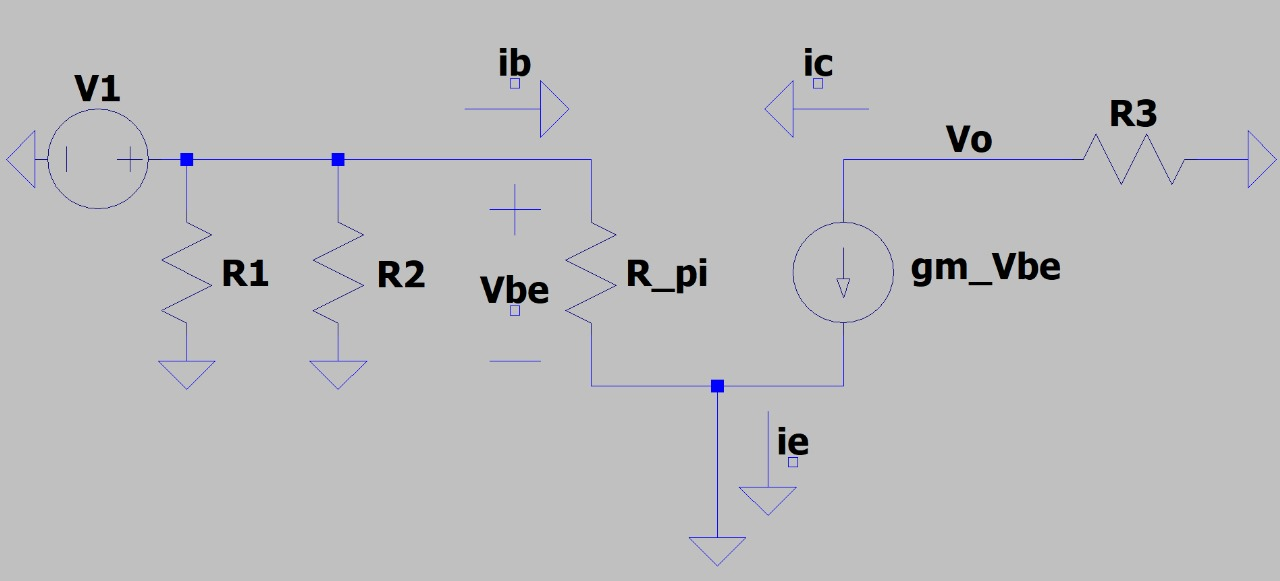
\includegraphics[width=0.6\columnwidth]{images/circuito_pequenos_sinais.png}
    \caption{Circuito com substituições para pequenos sinais.}
    \label{fig:circuito_pequenos_sinais}
\end{figure}

\subsubsection{Análise nodal do circuito}

Utiliza-se a lei de Kirchhoff das correntes para derivar as equações nodais seguintes.

\begin{equation}
    \begin{aligned}
        - I_{b} + \frac{V_{i}}{Rpi} = 0 \\
        I_{c} + \frac{V_{o}}{R_{c}} = 0 \\
        I_{c} - V_{be} gm = 0           \\
        - I_{b} - I_{c} + I_{e} = 0     \\
        I_{b} R_{\pi} - V_{be} = 0
    \end{aligned}
    \label{eq:analise_nodal_pequenos_sinais}
\end{equation}

\subsubsection{Ganho de tensão}

Para analisar o ganho de tensão, foi realizada uma solução numérica para $V_o$ e $V_i$, utilizando as equações \ref*{eq:analise_nodal_pequenos_sinais}. Os resultados obtidos são os seguintes:

\begin{equation}
    A = - gm R_c
\end{equation}

\subsubsection{Resistência de entrada}

Para analisar a resistência de entrada, foi realizada uma solução numérica para $V_i$ e $I_i$, utilizando as equações \ref*{eq:analise_nodal_pequenos_sinais}. Os resultados obtidos são os seguintes:

\begin{equation}
    R_{in} = R_{\pi}  //  R_1  //  R_2
\end{equation}

\subsubsection{Resistência de Thevenin}

Ao anular as fontes de tensão independentes, a tensão através de $R_{\pi}$ se torna zero, o que faz com que $V_{be0}$ seja igual a zero, desativando assim a fonte de corrente dependente.

Isso leva à conclusão de que a resistência de Thévenin é igual a $R_c$
.

\subsubsection{Tensão de Thevenin}

Analisa-se a tensao que esta sendo aplicada sobre $R_c$ e com isso obtemos que $V_{th} = V_o = V_c$.

\subsubsection{Constante de proporcionalidade}

Ao considerar $K = V_{th} / V_i$ e $V_{th} = V_o$, podemos afirmar que K é igual ao ganho de tensão que calculamos anteriormente.

\begin{equation}
    K = A = - gm R_c
\end{equation}


\subsection{Projeto do circuito}

Obtivemos $n_1 = n_2 = n_3 = n_4 = 1$. Assumindo que $V_{BE0} = 0.7 V$, $\beta = 350$, e $n V_r = 40 mV$, atendendo os requesitos calcula-se:

\begin{equation}
    \begin{aligned}
         & V_{cc} - \frac{V_{cc}}{4} = (100 + 50 n_1) n V_t \\
         & V_{cc} = 8                                       \\
         & V_{ee} = -8                                      \\
    \end{aligned}
\end{equation}

\begin{equation}
    \begin{aligned}
         & R_1 = \frac{(V_{cc} - V_b)  10}{I_c} = 11 k \varOmega \\
         & R_2 = \frac{- V_{cc} - V_b}{I_c} = 2.25 k \varOmega   \\
    \end{aligned}
\end{equation}

\begin{equation}
    \begin{aligned}
         & R_c = \frac{\left(V_{cc} - \frac{V_{cc}}{4}\right)}{2 (n_2 +5)} = 500\varOmega \\
         & R_e = \frac{V_e + V_{cc}}{I_e} = 167 \varOmega
    \end{aligned}
\end{equation}

Neste ponto, são feitas as seguintes aproximações para os valores dos resistores, considerando as opções disponíveis no mercado de componentes eletrônicos.

\begin{center}
    \begin{tabular}{ |c|c|c| }
        \hline
        Medidas & Experimental & Numerico   \\
        $T$     & $510.62 ms$  & $515.8 ms$ \\
        $k$     & $0.5$        & $0.501$    \\
        $V_1$   & $4.31V$      & $4.313V$   \\
        $V_2$   & $5.4V$       & $5.39V$    \\
        $I_L$   & $12.95mA$    & $12.95mA$  \\
        \hline
    \end{tabular}
\end{center}